\section{Introduction}

\hidenum
\begin{frame}[noframenumbering]
\frametitle{Contents}
 \tableofcontents[currentsection,hideallsubsections]
\end{frame}
\shownum

\subsection{pbdR}

\begin{frame}
  \begin{block}{Why R?}
    \pause
    \begin{enumerate}[<+-|alert@+>]
      \item Because.
      \item R community has growing data size problem.
      \item HPC community has growing need for data analytics.
    \end{enumerate}
  \end{block}
\end{frame}


\begin{frame}
  \begin{block}{Elevating R to Supercomputers}
  \pause
    \begin{enumerate}[<+-|alert@+>]
      \item Existing code.
      \item Syntax.
      \item Philosophy.
    \end{enumerate}
  \end{block}
\end{frame}


\begin{frame}
  \begin{block}{Programming with Big Data in R (pbdR)}
       \centering \emph{Productivity, Portability, Performance}\\[.4cm]
  \begin{columns}[onlytextwidth]
    \begin{column}{0.30\textwidth}
      \centering
       
\includegraphics[width=3.4cm]{pics/simple}\\[.2cm]
    \end{column}
    \begin{column}{0.65\textwidth}
  \begin{itemize}
    \item \emph{Free}\footnote{MPL, BSD, and GPL licensed} R packages.
    \item Bridging high-performance C with high-productivity of R
%     \item Scalable, big data analytics.
    \item Distributed data details implicitly managed.
    \item Methods have syntax \emph{identical} to R.
%     \item Powered by state of the art numerical libraries (MPI, ScaLAPACK, \dots)
  \end{itemize}
    \end{column}
​  \end{columns}
\end{block}
\end{frame}



\begin{frame}
  \begin{block}{pbdR Packages}
    \begin{center}
%         \includegraphics[width=7cm, height=7cm]{pics/pbdpacks}
      \begin{columns}
        \begin{column}{.52\textwidth}
      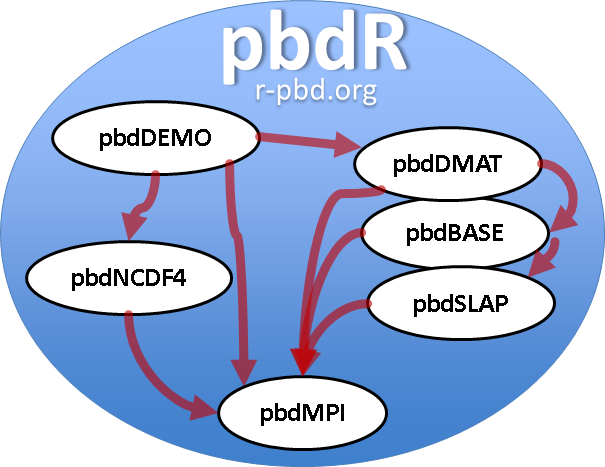
\includegraphics[scale=.4]{pics/pbdR}
        \end{column}
        \hfill
        \begin{column}{.4\textwidth}
      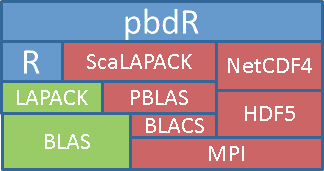
\includegraphics[scale=.45]{pics/libs}
        \end{column}
      \end{columns}
    \end{center}
  \end{block}
\end{frame}


\begin{frame}[fragile]
\begin{block}{pbdMPI vs Rmpi}
\pause
\begin{lstlisting}[title=Reduce Operation with Rmpi]
# int
mpi.allreduce(x, type=1)
# double
mpi.allreduce(x, type=2)
\end{lstlisting}

\begin{lstlisting}[title=Reduce Operation with pbdMPI]
allreduce(x)
\end{lstlisting}

\pause
\begin{lstlisting}
> is.integer(1)
[1] FALSE
> is.integer(2)
[1] FALSE
> is.integer(1:2)
[1] TRUE
\end{lstlisting}
\end{block}
\end{frame}


\begin{frame}
\begin{block}{pbdMPI vs Rmpi}
\begin{table}[h]
 \centering
 \caption{Runtimes (seconds) for $10,000 \times 10,000$ \code{allgather} with \pkg{Rmpi} and \pkg{pbdMPI}.}
 \label{tab:allgather}
 \begin{tabular}{rrrr}\hline\hline
  Cores & \pkg{Rmpi} & \pkg{pbdMPI} & Speedup \\\hline
  32    & 24.6       & 6.7          & 3.67 \\
  64    & 25.2       & 7.1          & 3.55 \\
  128   & 22.3       & 7.2          & 3.10 \\
  256   & 22.4       & 7.1          & 3.15 \\\hline\hline
 \end{tabular}
\end{table}
\end{block}
\end{frame}



\begin{frame}[fragile]
  \begin{block}{pbdR Example Syntax}
  \begin{lstlisting}
x <- x[-1, 2:5]
x <- log(abs(x) + 1)
xtx <- t(x) %*% x
ans <- svd(solve(xtx))
  \end{lstlisting}
  \begin{center}
  Look familiar?\\[.4cm]
  \emph{The above runs on 1 core with R or 10,000 cores with pbdR}
  \end{center}
  \end{block}
\end{frame}

